%
% File acl2014.tex
%
% Contact: giovanni.colavizza@epfl.ch
%%
%% Based on the style files for ACL-2013, which were, in turn,
%% Based on the style files for ACL-2012, which were, in turn,
%% based on the style files for ACL-2011, which were, in turn, 
%% based on the style files for ACL-2010, which were, in turn, 
%% based on the style files for ACL-IJCNLP-2009, which were, in turn,
%% based on the style files for EACL-2009 and IJCNLP-2008...

%% Based on the style files for EACL 2006 by 
%%e.agirre@ehu.es or Sergi.Balari@uab.es
%% and that of ACL 08 by Joakim Nivre and Noah Smith

\documentclass[11pt]{article}
\usepackage{acl2014}
\usepackage{times}
\usepackage{url}
\usepackage{latexsym}
\usepackage{graphicx}
\usepackage{nicefrac}
\graphicspath{ {./images/} }

%\setlength\titlebox{5cm}

% You can expand the titlebox if you need extra space
% to show all the authors. Please do not make the titlebox
% smaller than 5cm (the original size); we will check this
% in the camera-ready version and ask you to change it back.


\title{Smart recipes}

\author{Omar Mehio \\
  {\tt\small omar.mehio@epfl.ch} \\\And
  Leonardo Perrone \\
  {\tt\small leonardo.perrone@epfl.ch} \\\And
  Attila Bekker \\
  {\tt\small attila.bekker@epfl.ch} \\}

\date{16th of December, 2018}

\begin{document}
\maketitle
\begin{abstract}
  The aim of this document is to find correlations between attributes and characteristics of food recipes and the corresponding ratings and reviews given to that recipe.
  
  Recipes are gathered from the most popular online recipe websites, extracting common attributes and normalizing them between the different representations. Apart from the attributes explicitly included in the recipe descriptions, new properties are being defined by grouping recipe ingredients into different categories. Furthermore, sentiment analysis is performed on the content of recipe reviews, providing a way to determine the corresponding ratings.
  
  Performing a range of different analysis techniques provides a set of hints and best practices to help recipe authors to maximize their ratings by choosing the recipes with attributes most likely to be rated positively.
\end{abstract}

\section{Introduction}

This document has been prepared for the \textbf{Applied Data Analytics} course at EPFL in the Fall of 2018.

\section{Data acquisition}

The recipe data has been extracted from the \textit{Cooking recipes} database, which is a collection of HTML documents from a wide variety of websites.

\subsection{Data sources}

The analysis has been based on data extracted from the most popular websites containing food recipes. The data included recipes from over 50 websites, all featuring their own custom format and attributes. Since each website required a custom scraper to be built, and each website displays different attributes of recipes and their ingredients, the aim was to select a small number of websites which still offer a good representation of the entire data set. The aim was to work with \nicefrac{2}{3} of the total number of available recipes.

\vspace{5mm}
\begin{center}
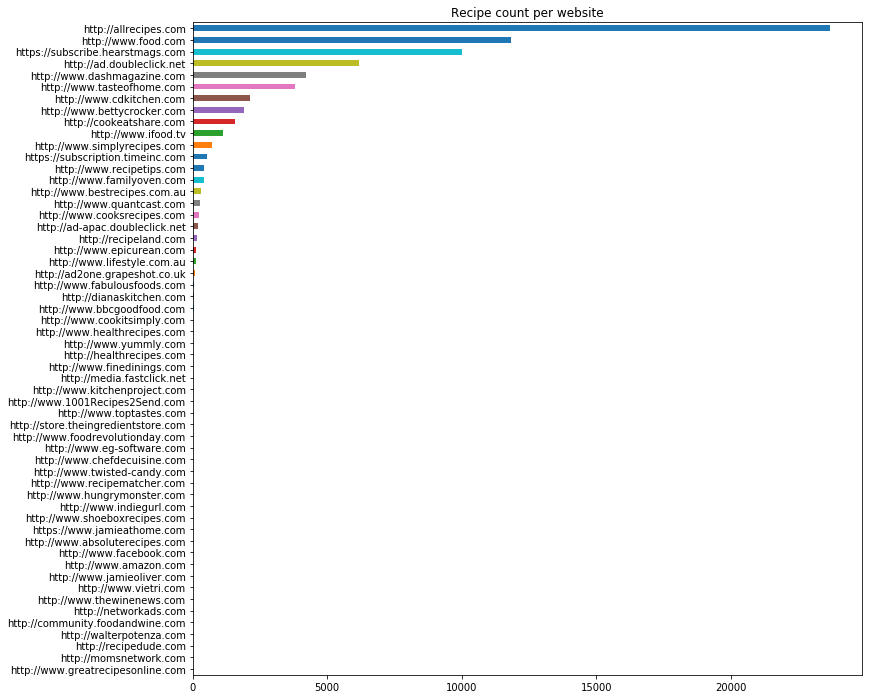
\includegraphics[scale=0.22]{website-count}
\label{website-count} Figure 1. Recipe count
\end{center}
\vspace{5mm}

The top 3 websites containing the most recipes cover about 65\% of all data: 
\begin{enumerate}
\item http://allrecipes.com
\item http://www.food.com
\item https://subscribe.hearstmags.com (food-net)
\end{enumerate}

\subsection{Data import}

The three selected websites provided different recipe attributes in different formats, which needed to be parsed and consolidated into a common format in order to perform meaningful analysis on them.
Common attributes were:
\begin{itemize}
    \item name
    \item review text
    \item review date
    \item rating
    \item category
    \item ingredient list
    \item nutritional values
    \item preparation time
    \item cooking time
    \item difficulty
    \item serving size
\end{itemize}
These attributes may have different scales, different measurement units, or may be missing altogether. 

The three websites required custom scraping algorithms. The source data volume was about 13 GB, making it feasible to be processed on a single computer. The scraping took 20-30 minutes, the results were stored in \textit{json} format to allow efficient processing.

\subsection{Data cleaning}

Due to the different formats, the data sets had to be cleaned separately. Nutrition information had to be converted to numeric values on a unified scale, using the same measurement units across all recipes. Time values expressed in hours or days needed to be converted to minutes. Rating values had to be scaled to a common range. Some text values had to be converted to numeric values.

\subsection{Review pre-processing}

The content of the reviews had special importance for the analysis. In order to analyze the text, a pipeline was constructed to clear the text. Numbers and other non-alphanumeric characters were removed, and all remaining text was converted to lowercase. Stop words offered little value in terms of semantic analysis, so they were removed. Lemmatizing removed prefixes and suffixes, helping to group similar words. Finally a document term matrix was constructed using both TF-IDF and one-hot encoding matrices.

\section{Preliminary visual analysis}

Once the raw data had been converted into a clean data set with common attributes, they were visualized in order to better understand the characteristics. This analysis was performed before combining the data sets into a single one, allowing comparison between websites.

\subsection{Ratings}

Ratings were found to be dominated by high values. After converting them to a common scale of 3 it was observed that good ratings highly outnumber bad or medium ones.

\vspace{5mm}
\begin{center}
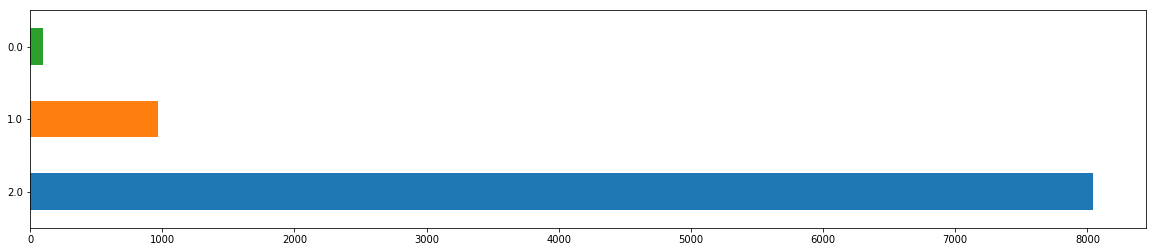
\includegraphics[scale=0.085]{ratings-1}
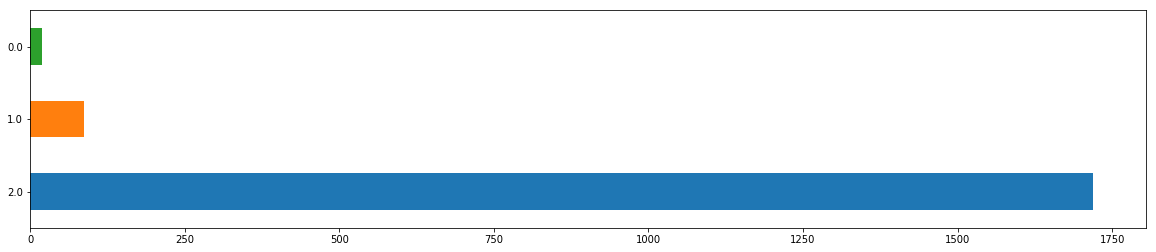
\includegraphics[scale=0.085]{ratings-2}
\label{visalization-ratings} Figure 2. Ratings distribution
\end{center}
\vspace{5mm}

\subsection{Serving size}

Serving sizes ranged up to 300, but there were only a small number of recipes for more than 50 persons. The 75\% percentile fell to serving sizes of 8 and 12 respectively for the two websites with the most recipes. 

\vspace{5mm}
\begin{center}
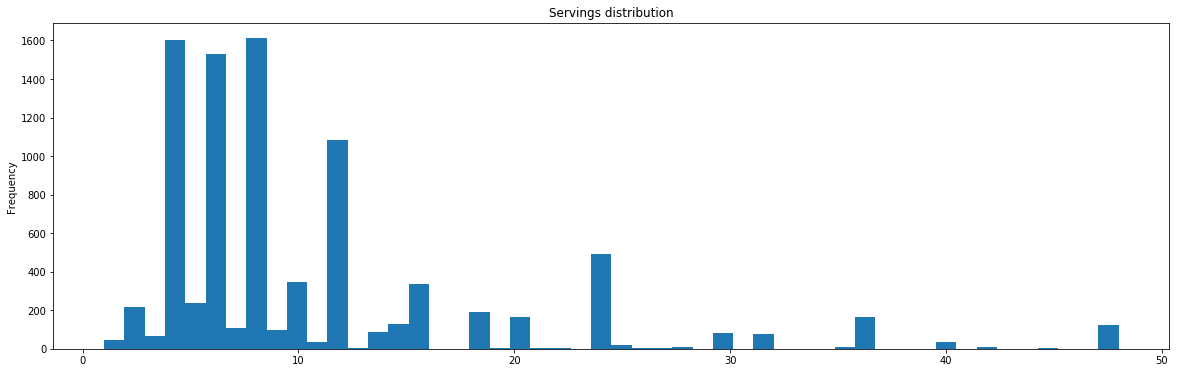
\includegraphics[scale=0.085]{servings-1}
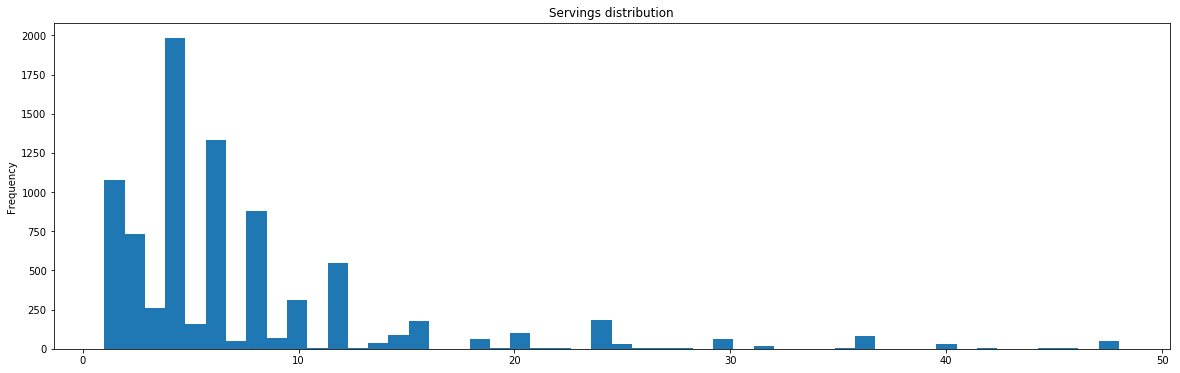
\includegraphics[scale=0.085]{servings-2}
\label{visalization-servings} Figure 3. Servings distribution
\end{center}
\vspace{5mm}

\subsection{Reviews over time}

Most reviews have been created between 2000 and 2010, indicating the period when the data had been collected. The density curves suggested different trends for the popularity of the websites. The allrecipes site showed declining review numbers over the years, while food.com had fairly constant activity, and food-net reviews sharply increased towards the end of the period.

\vspace{5mm}
\begin{center}
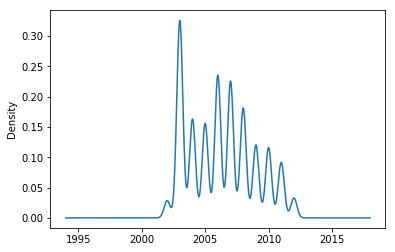
\includegraphics[scale=0.17]{time-1}
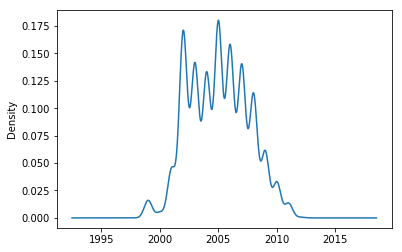
\includegraphics[scale=0.17]{time-2}
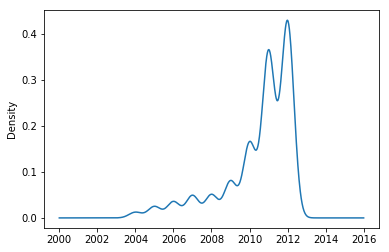
\includegraphics[scale=0.17]{time-3}
\label{visalization-time} Figure 4. Reviews over time
\end{center}
\vspace{5mm}

\subsection{Cooking time}

Cooking times ranged from a few minutes to several hours, but the distribution showed that most recipes required less than 1 hour cooking, recipes requiring 30 minutes or less being the most common.

\vspace{5mm}
\begin{center}
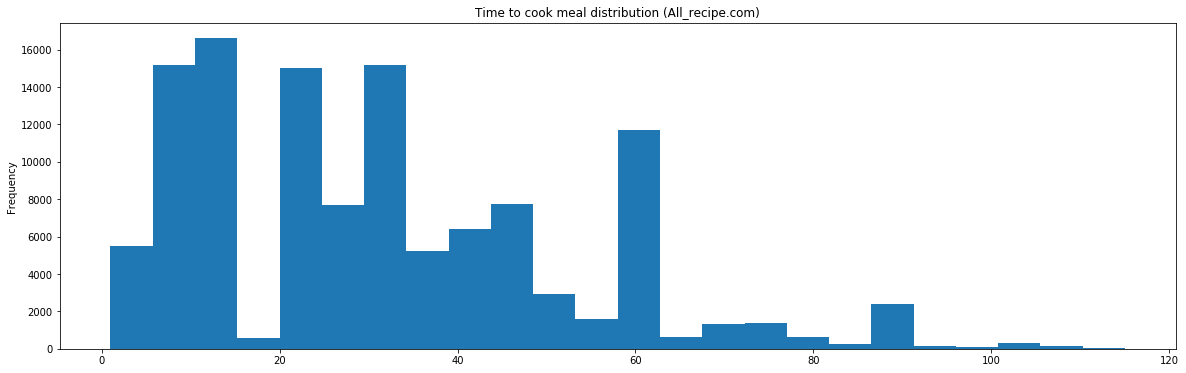
\includegraphics[scale=0.06]{cookingtime-1}
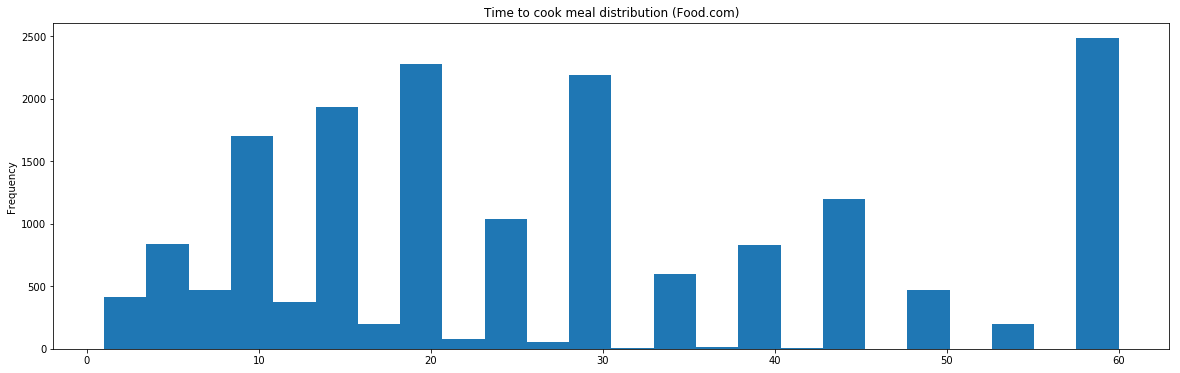
\includegraphics[scale=0.06]{cookingtime-2}
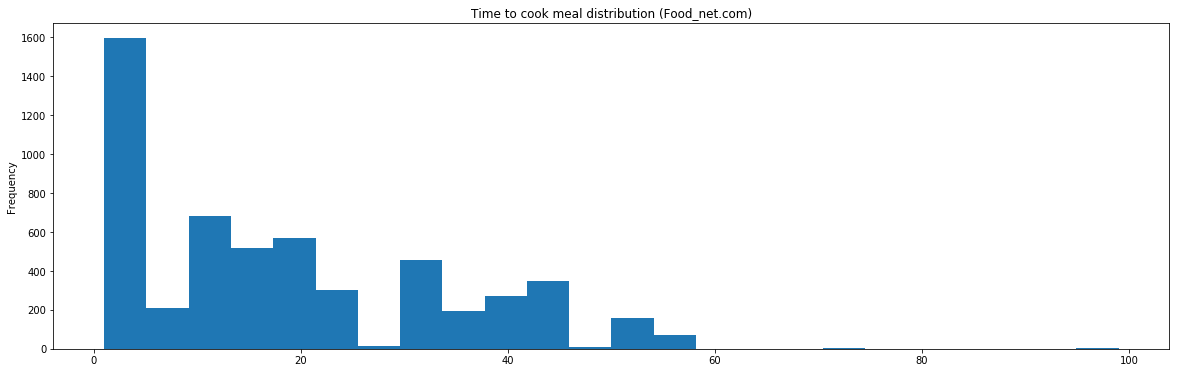
\includegraphics[scale=0.06]{cookingtime-3}
\label{visalization-cookingtime} Figure 5. Cooking time distribution
\end{center}
\vspace{5mm}

\section{Ingredient clustering}

Comparing recipes based on ingredients is problematic, due to the high number of possible ingredients. By grouping similar ingredients into clusters we were able classify recipes by how many ingredients they contained from each cluster. The following procedure has been performed separately for the different websites, for the sake of simplicity we demonstrate the results from food.com only.

First, measurements and other non-food related words needed to be removed from the review text. For example, words like cup or tablespoon were featured frequently, but were irrelevant to define ingredient clusters. Removing these words and keeping only ingredients resulted in more balanced distribution.

\vspace{5mm}
\begin{center}
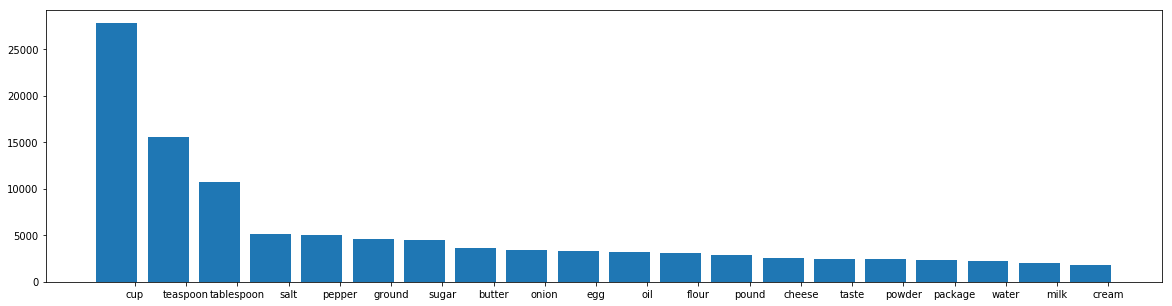
\includegraphics[scale=0.18]{ingredient-before}
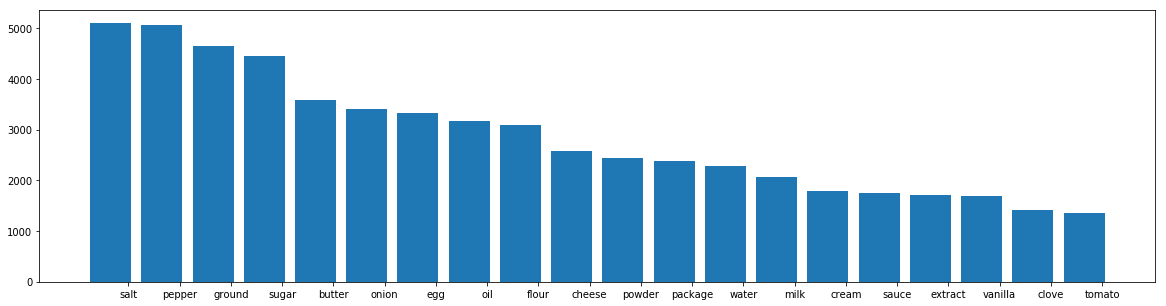
\includegraphics[scale=0.18]{ingredient-after}
\label{visalization-cookingtime} Figure 6. Ingredient distribution
\end{center}
\vspace{5mm}

By applying pre-trained word2vec vectors, we mapped each ingredient into a word vector, and projected them to a 2-dimensional plane using t-distributed stochastic neighbor embedding. 

\vspace{5mm}
\begin{center}
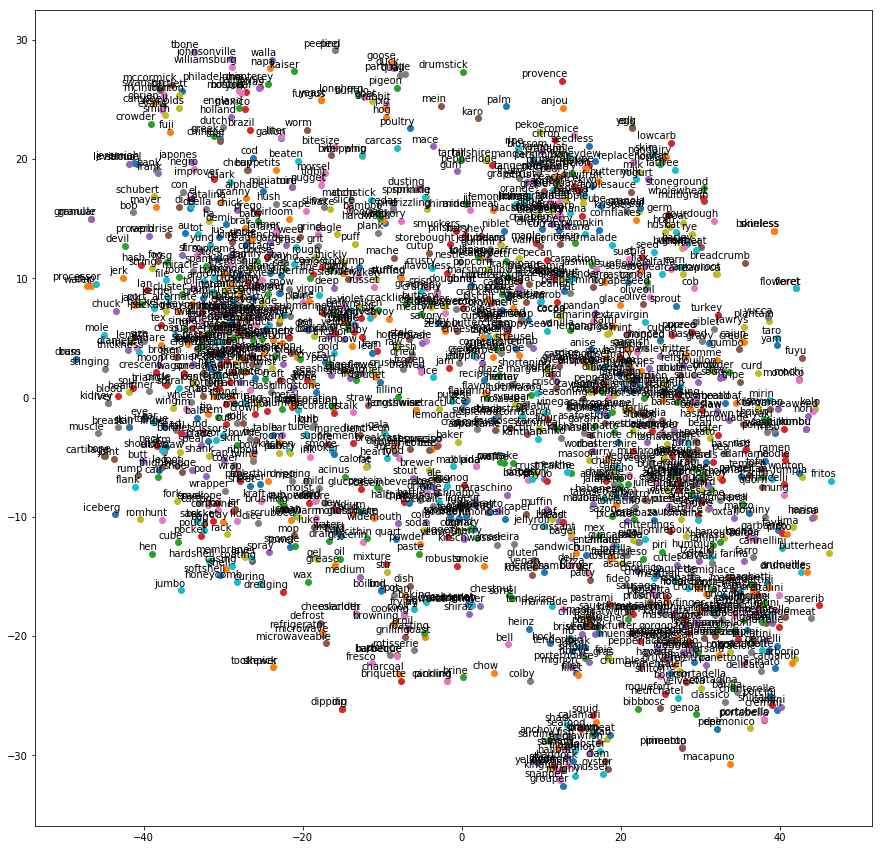
\includegraphics[scale=0.24]{ingredient-tsne}
\label{visalization-cookingtime} Figure 7. Ingredient word vectors
\end{center}
\vspace{5mm}

We used silhouette analysis to find the optimal number of clusters for the k-means clustering, determining that 29 clusters produced the best performance.

\vspace{5mm}
\begin{center}
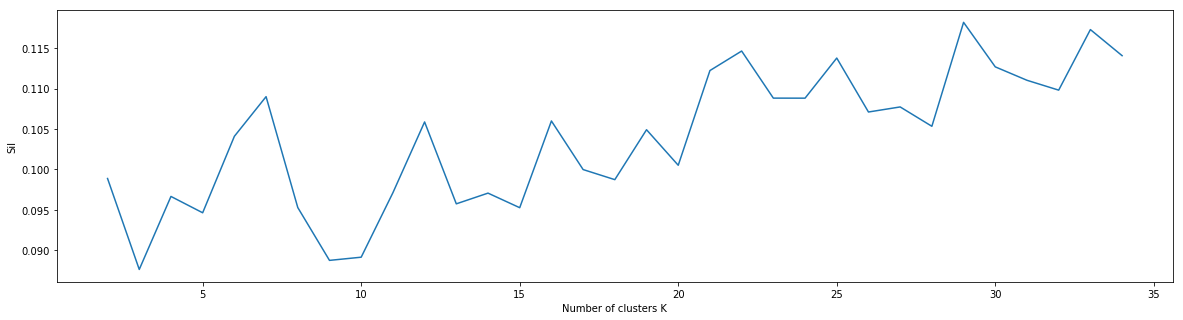
\includegraphics[scale=0.18]{ingredient-kmeans}
\label{visalization-cookingtime} Figure 8. K-means silhouette analysis
\end{center}
\vspace{5mm}

Based on manual analysis of the classified ingredients, the individual clusters have been named accordingly and projected on the 2D plane.

\vspace{5mm}
\begin{center}
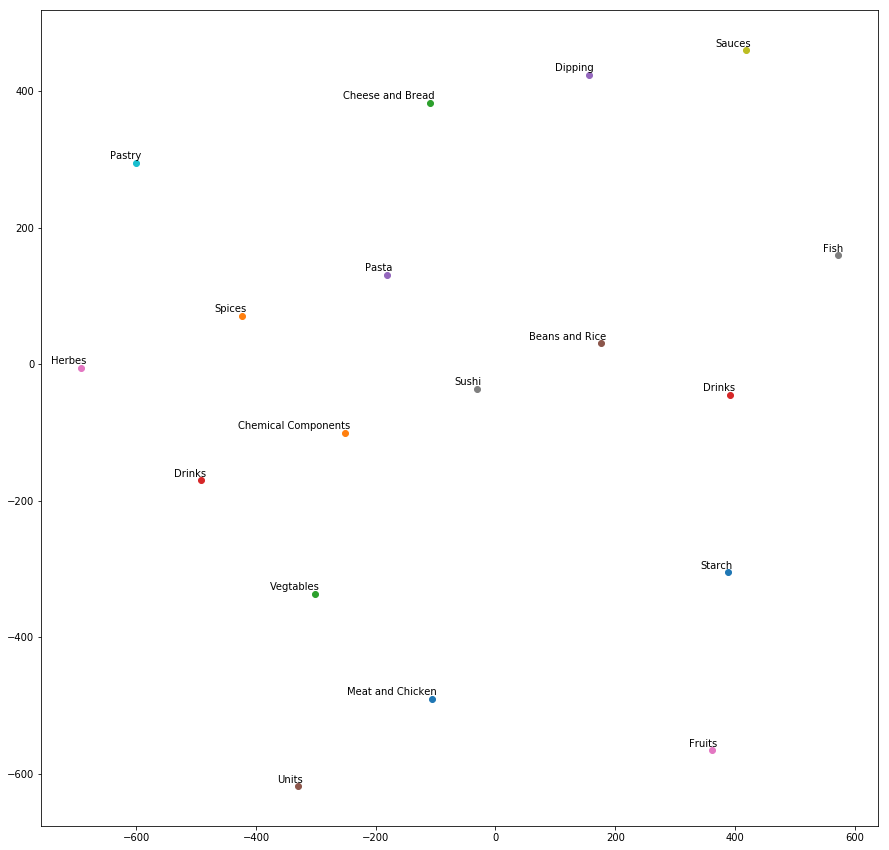
\includegraphics[scale=0.24]{ingredient-clusters}
\label{visalization-cookingtime} Figure 9. Ingredient clusters
\end{center}
\vspace{5mm}

\section{Unified data set}

The next step was to combine the cleaned and pre-processed data from the three websites into a single unified data set, and prepare the attributes so they can be efficiently analyzed.

\subsection{Missing ratings}

Since ratings had special importance for the study, keeping the values on a scale from 1 to 5 allowed more fine grained evaluation rather than compressed ratings on a 1 to 3 scale which was used for the preliminary analysis.

\vspace{5mm}
\begin{center}
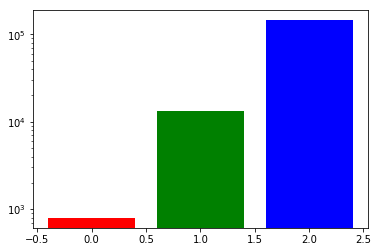
\includegraphics[scale=0.25]{rating-1-to-3}
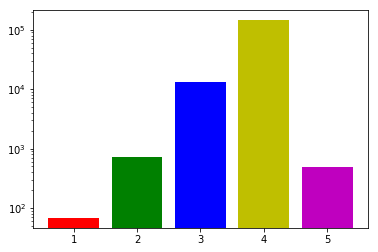
\includegraphics[scale=0.25]{rating-1-to-5}
\label{visalization-cookingtime} Figure 10. Rating distribution on scales of 3 and 5
\end{center}
\vspace{5mm}

The food-net site contained no rating values at all, only reviews. In order to retain this data, the missing rating values had to be enriched based on the reviews. This has been achieved by using sentiment analysis and logistic regression where both reviews and ratings were available, and use the trained model to predict the missing rating values from the corresponding reviews.

\subsection{Rating bias}

Rating values of 4 were by far the most common, resulting in an implicit bias in the analysis. In order to reduce this bias, the first data set has been oversampled for the logistic regression training, so predicting the missing ratings resulted in a slightly more balanced distribution.

\vspace{5mm}
\begin{center}
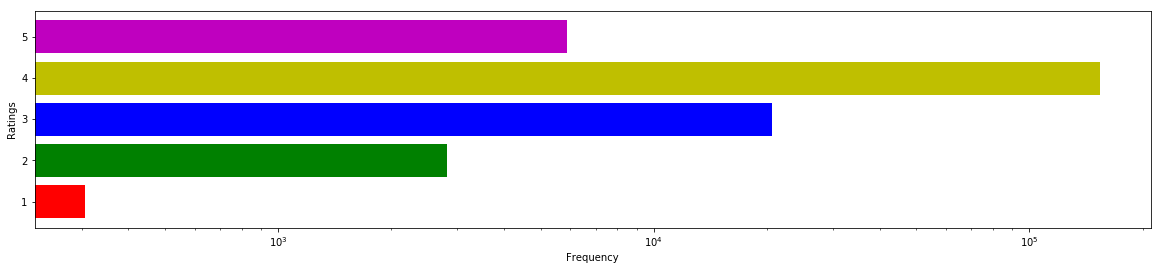
\includegraphics[scale=0.18]{rating-balanced}
\label{visalization-cookingtime} Figure 11. Improved rating balance
\end{center}
\vspace{5mm}

\subsection{Healthiness}

In order to determine how healthy a particular recipe is, the nutrition values have been compared with the commonly recommended daily intake values. Each recipe has been assigned a health grade, based on how many nutrients remain under 50\% of the recommended daily limit in a single serving. Most recipes received a health grade of 3 or 4 on a scale of 6.

\vspace{5mm}
\begin{center}
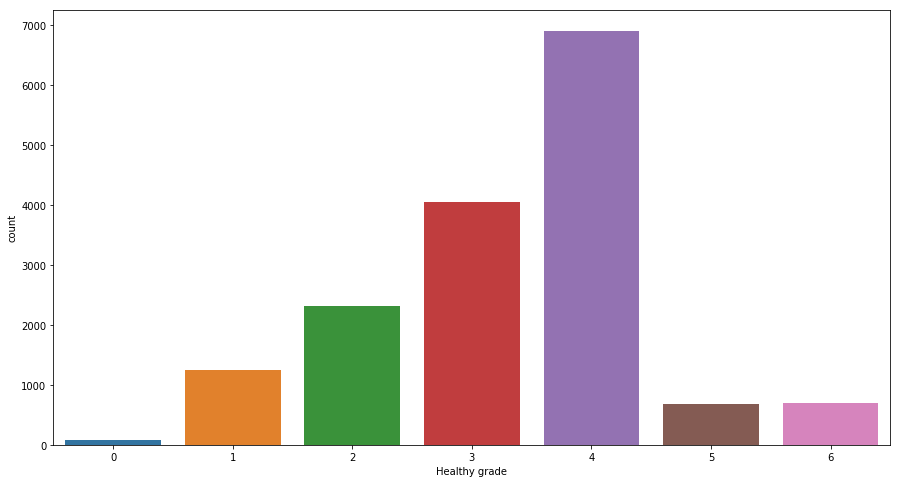
\includegraphics[scale=0.22]{health-grade}
\label{visalization-cookingtime} Figure 12. Health grades
\end{center}
\vspace{5mm}

\section{Analysis}

With the data converted to the same format and unified into a single data set, the analysis could be performed in order to establish which factors are most likely to influence positive reviews and ratings.






\begin{thebibliography}{}

\bibitem[2004]{FDA:04}
{U.S. Food and Drug Administration}
\newblock 2004.
\newblock {\em How to Understand and Use the Nutrition Facts Label, The Percent Daily Value (\%DV)}
\newblock {https://www.fda.gov/food/labelingnutrition/ \\ ucm274593.htm\#percent\_daily\_value}

\bibitem[2007]{ABC:07}
{ABC Healh and Wellbeing}.
\newblock 2007.
\newblock {\em What is a healthy recipe?}.
\newblock {http://www.abc.net.au/health/library/ \\
stories/2007/04/23/1904178.htm}

\end{thebibliography}

\end{document}
